Η υλοποίηση του συστήματος ανίχνευσης εισβολών (IDS) βασίζεται στη δημιουργία μιας ολοκληρω-μένης υποδομής, η οποία περιλαμβάνει client-server αρχιτεκτονική, τη χρήση του εργαλείου \textbf{Zeek} για την ανίχνευση εισβολών, καθώς και τη διαχείριση δεδομένων και τη δοκιμή επιθέσεων μέσω αυτοματοποιημένων και χειροκίνητων σεναρίων. Όλα τα μέρη της υποδομής αναπτύχθηκαν με γνώ-μονα τη χρήση \textbf{containerization}, ώστε να εξασφαλιστεί η ευκολία εγκατάστασης, διαχείρισης και παραμετροποίησης.

Η γενική τοπολογία περιλαμβάνει τρεις βασικούς πυλώνες: τον client, τον server και το \textbf{Zeek-based} IDS. Ο client αποτελεί το frontend της υποδομής μας και είναι υπεύθυνος για την αλληλεπίδραση με τον χρήστη. Περιλαμβάνει στατικά αρχεία \textbf{HTML}, \textbf{CSS} και \textbf{JavaScript}, τα οποία φιλοξενούνται μέσω ενός container που λειτουργεί με \textbf{Nginx}. Αυτή η πλευρά του συστήματος επιτρέπει στον χρήστη να στέλνει αιτήματα και να προσομοιώνει διαφορετικά σενάρια επιθέσεων, όπως SQL Injection ή \textbf{Cross-Site Scripting} (\textbf{XSS}).

Ο server υλοποιήθηκε με τη χρήση της γλώσσας \textbf{Go}, η οποία προσφέρει υψηλή απόδοση και ασφάλεια στη διαχείριση αιτημάτων. Λειτουργεί ως ο μεσάζων ανάμεσα στον client και τα υπόλοιπα υποσυστήματα, επεξεργάζεται τα εισερχόμενα δεδομένα και αποθηκεύει τις πληροφορίες σε μια βάση δεδομένων \textbf{MySQL}. Το αρχείο \textbf{setup.sql} περιλαμβάνει τις αρχικές ρυθμίσεις της βάσης, ενώ ο κώδικας του server (main.go) έχει σχεδιαστεί για να δέχεται τόσο έγκυρα όσο και κακόβουλα αιτήματα, διευκολύ-νοντας τη δοκιμή των κανόνων του \textbf{Zeek}.

Στον πυρήνα του συστήματος βρίσκεται το \textbf{Zeek}, το οποίο έχει παραμετροποιηθεί να λειτουργεί σε περιβάλλον \textbf{Docker}. Το \textbf{Zeek} είναι υπεύθυνο για την παρακολούθηση της δικτυακής κίνησης που διέρχεται από τον server. Οι κανόνες ανίχνευσης, που είναι ορισμένοι στο αρχείο \textbf{alerts.zeek}, σχεδιάστηκαν για να εντοπίζουν συγκεκριμένα μοτίβα επιθέσεων, όπως \textbf{DDoS}, \textbf{SQL Injection} και \textbf{Path Traversal}. Το εργαλείο είναι επίσης ρυθμισμένο να εξάγει δεδομένα και alerts, τα οποία καταγρά-φονται στη βάση δεδομένων για περαιτέρω ανάλυση.

\begin{figure}[H]
\centering
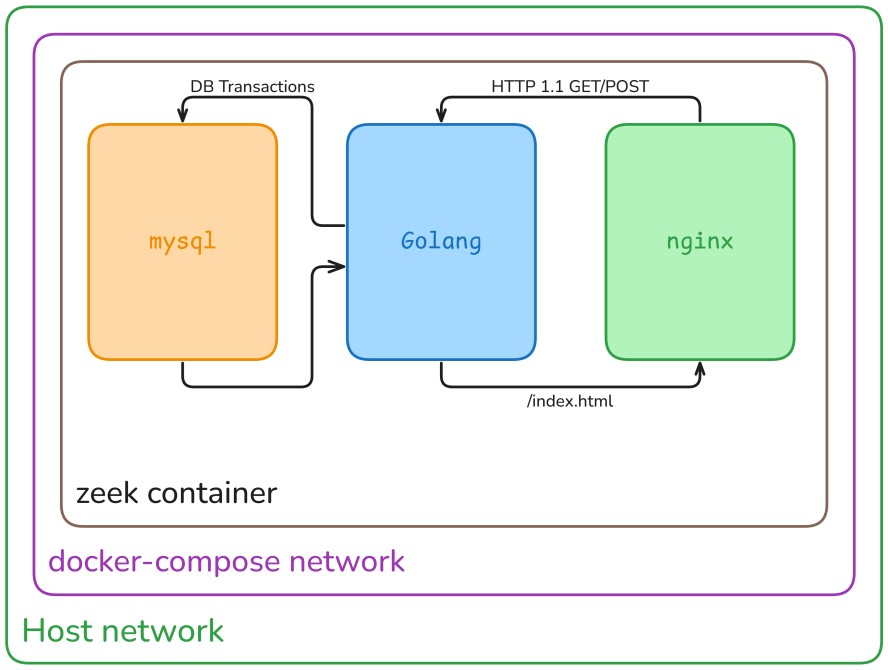
\includegraphics[width=0.7\textwidth]{image}
\caption*{\small{\textbf{Εικόνα 2.1.1} Γενική επισκόπηση της προτεινόμενης αρχιτεκτονικής}}
\end{figure}

Όλα τα παραπάνω υποσυστήματα είναι συνδεδεμένα μέσω ενός \textbf{docker-compose} αρχείου, το οποίο ρυθμίζει την επικοινωνία ανάμεσα στα containers. Το \textbf{Zeek} λειτουργεί ως το κεντρικό IDS, ενώ ο server και ο client είναι υπεύθυνοι για τη διαχείριση και την εκτέλεση αιτημάτων. Η παρακολούθηση των δικτυακών αιτημάτων και η ανταπόκριση του συστήματος γίνεται σε πραγματικό χρόνο, επιτρέπο-ντας την ανάλυση της απόδοσης των κανόνων ανίχνευσης και την αξιολόγηση της λειτουργικότητας του συστήματος.

Με αυτήν την υποδομή, καταφέραμε να δημιουργήσουμε ένα ολοκληρωμένο περιβάλλον, το οποίο είναι επεκτάσιμο και ευέλικτο, τόσο για τη δοκιμή νέων κανόνων ανίχνευσης όσο και για την προσομοί-ωση διαφορετικών σεναρίων εισβολής.
